\section{Das iOS Betriebsystem}
	Die aus Cupertino in Kalifornien stammende US-Amerikanische Apple Corporation
	ist eine der größten Firmen der Welt und hatte einen Umsatz von 182 Mrd.
	USD im Geschäftsjahr 2014. Sie ist ebenfalls der Erfinder des mobilen
	Betriebssystems iOS, welches auf den firmeneigenen Geräten iPad, iPad mini,
	iPhone, iPod touch und dem Apple TV ab der zweiten Generation zum Einsatz
	kommt. Als Steve Jobs 1985 das Unternehmen verließ, gründete er
	kurze Zeit darauf die Firma NeXT, mit welcher er unter anderem das
	Betriebsystem NeXTStep entwickelte, welches auf dem UNIX ähnlichem
	Betriebsystem BSD\cite{Tanenbaum2009} und dem	Mach-2.5-Kernel
	\footnote{http://www.cs.cmu.edu/afs/cs/project/mach/public/www/mach.html}
	basiert. NeXT wurde 1996 von Apple aufgekauft und Jobs kehrte als neuer CEO zu
	Apple zurück. Damit begann die Karriere des mobilen Betriebsystems. Zuerst
	wurde NeXTStep als Portierung in Form von Mac OS X, später OS X weiter
	entwickelt. Mac OS X ist wiederrum der Vorleger für iPhone OS, später iOS,
	welches am 09.Januar 2007 mit dem damals neu erschienenen iPhone erstmals
	vorgestellt wurde. Im März 2015 hatte iOS in den USA einen Marktanteil von
	36,5\% und 18,3\% in Deutschland.
	\footnote{http://www.kantarworldpanel.com/global/smartphone-os-market-share/}\\
	
	\begin{figure}[h]
		\centering
		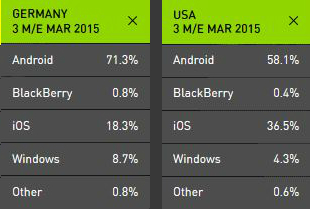
\includegraphics[width=0.5\linewidth]{ios/media/marketshare-cmp-201503.jpg}
		\caption{Marktanteil der Smartphone Betriebssysteme
		\cite{MobileOsStat}}
		\label{fig:marcetshare}
	\end{figure}